\documentclass[8pt]{beamer}
\usepackage{tikz}
\usepackage[utf8]{vietnam}
\usepackage{amsmath}
\usepackage{graphicx}
\usepackage{wrapfig}
\usepackage{hyperref}
\usetheme{Copenhagen}
\usecolortheme{beaver}
\setbeamertemplate{navigation symbols}{}
\setbeamertemplate{headline}{}
\title[Chương 0: Giới thiệu môn học] %optional
{Chương 0: Giới thiệu môn học}
\subtitle{Tín hiệu và hệ thống}
\author[Tín hiệu và hệ thống] % (optional)
{Tín Vũ}
\date[VLC 2021] % (optional)
{tinvu1309@gmail.com}
\begin{document}
\frame{\titlepage}
\begin{frame}{Mục lục}
\tableofcontents
	\begin{enumerate}
		\item Giới thiệu playlist
		\item Giới thiệu khái quát môn học
		\item Kiến thức cơ sở tiên quyết
		\item Phương pháp học đúng
		\item Tài liệu tham khảo
		\item Ôn tập số phức (optional)
			\begin{itemize}
				\item Các phép toán cơ bản với số phức 
					\begin{itemize}
						\item Mặt phẳng phức
						\item Đồng nhất thức Euler
					\end{itemize}
				\item Ý nghĩa của số phức trong Vật lý
					\begin{itemize}
						\item Dao động điều hòa
						\item Mạch RLC
					\end{itemize}
				\item Tại sao lại dùng số phức để biểu diễn tín hiệu ?
			\end{itemize}
	\end{enumerate}
\end{frame}
\begin{frame}{Giới thiệu playlist}
	\begin{itemize}
		\item Mình là Tín Vũ, hiện tại đang là sinh viên học tại Trường Đại học Công nghệ, Đại học Quốc gia Hà Nội. Mình tạo playlist video này để hỗ trợ các bạn học môn Tín hiệu và hệ thống trong các trường đại học kĩ thuật theo hướng \alert{trực quan hóa} nhất có thể.
		\item Do đó, mục tiêu của mình khi thực hiện playlist này không chỉ giúp các bạn ôn thi được điểm cao mà còn \alert{hiểu sâu công thức để làm nền tảng cho các môn học sau}.
		\item Để đạt được hai mục tiêu trên, các bạn nên xem \textbf{toàn bộ} video của mình, còn nếu chỉ cần ôn thi cấp tốc và đạt điểm cao thì hãy \textbf{bỏ qua} các video "optional".
		\item Nội dung playlist này chủ yếu bám sát nội dung môn học Tín hiệu và hệ thống tại trường của mình; nếu các bạn học trường khác, hãy tham khảo kĩ đề cương hay đề thi của trường bạn để đối chiếu sao cho ôn tập đúng trọng tâm và hợp lý. 
		\item Môn học này bao gồm \textbf{6} chương, các chương đều liên quan rất chặt chẽ và logic với nhau nên hãy học cẩn thận ngay từ \alert{chương 0} để ôn thi cuối kì đỡ vất vả.
	\end{itemize}
\end{frame}
\begin{frame}{Giới thiệu khái quát môn học}
\begin{wrapfigure}{l}{0.4\textwidth} %this figure will be at the right
    \centering
    
\includegraphics[width=0.4\textwidth]{linux.jpg}
\end{wrapfigure}
"What is life?" \\"Everything is File." \\ - Average Linux nerd philosophy's about life.
\end{frame}
\begin{frame}{Giới thiệu khái quát môn học}
\begin{wrapfigure}{l}{0.4\textwidth}
	\centering
	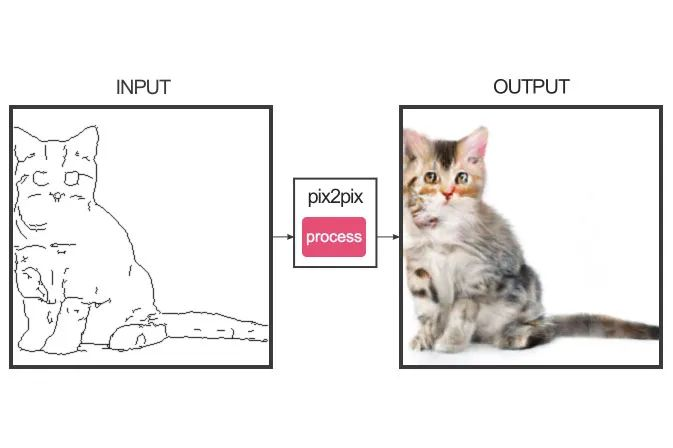
\includegraphics[width=0.4\textwidth]{cat.jpg}
\end{wrapfigure}
"Why is everything File?"
\\ "Because everything can mathematically be represented as an I/O mechanism - which is exactly how the \textbf{Signals and Systems} model works. If I know its function, I can predict the \textbf{future}."
\\ - Me in real life.
\end{frame}
\begin{frame}{Giới thiệu khái quát môn học}
\begin{itemize}
	\item Tất cả các hệ thống vật lý trong tự nhiên đều có thể được biểu diễn bằng mô hình \textbf{Signals and Systems} như sau:
		\begin{figure}[h]
			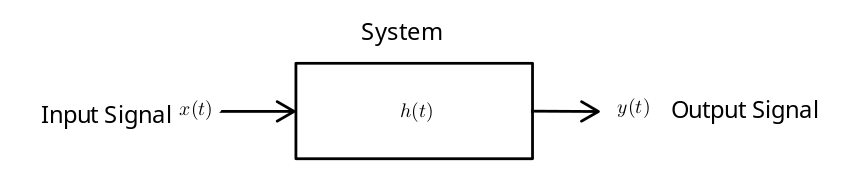
\includegraphics[width=0.75\textwidth]{model.png}
			\caption{Signal and System model}
			\label{fig:re2}
		\end{figure}
	\item Ví dụ như: khi các bạn bật điện, tín hiệu cơ học (input signal) sẽ đi qua một hệ thống điện (system) để kích hoạt tín hiệu điện (output signal) làm đèn sáng; khi các bạn lấy tay 
đấm vào tường (don't do it bro), lực từ nắm tay của các bạn (input signal) sau khi đi qua bức tường (system) sẽ trả về một lực phản hồi từ bức tường theo định luật III Newton (output signal) khiến cho tay bị đau. \\	$\Rightarrow$ Và còn vô số các ví dụ khác trong thực tiễn cuộc sống...
\item Môn học này sẽ tập trung đi sâu vào tìm hiểu các mối quan hệ cơ bản giữa \textbf{Tín hiệu} và \textbf{Hệ thống} bằng cách sử dụng mô hình toán học như phương trình vi phân, sơ đồ khối để trả lời các câu hỏi như: Làm thế nào để biết được tín hiệu ra của hệ thống ? Tín hiệu được cấu tạo từ những cái gì ? Ta có thể tạo ra hệ thống nào đó để điều khiển tín hiệu vào/ra theo ý muốn không ?
\end{itemize}
\end{frame}
\begin{frame}{Giới thiệu khái quát môn học}
	Một trong những ứng dụng cực kì tiêu biểu và phổ thông nhất của môn này đó là thiết kế bộ \textbf{lọc} tín hiệu. Hãy tưởng tượng các bạn là phóng viên thể thao đang tường thuật trực tiếp một trận bóng đá, ở sân bóng người ta thường sử dụng còi và hò hét rất ồn. Vậy làm thế nào để bạn có thể \textbf{lọc} được tất cả các âm thanh nhiễu (noise) đó để khán giả xem truyền hình vẫn có thể nghe được tiếng của bạn nói? Để giải quyết bài toán này, chúng ta cần phải trả lời các câu hỏi sau đây:
	\begin{itemize}
		\item Tín hiệu trước và sau khi lọc được cấu tạo từ những cái gì (hay những phần tử nào) ?
		\item Sau khi đã trả lời được câu hỏi trên, ta có thể tạo ra hệ thống để điều khiển tín hiệu vào/ra theo ý muốn không ?
		\item Cuối cùng, sau khi đã tạo ra được hệ thống thì làm thế nào ta có thể biết được đầu ra của nó? Đầu ra của nó có \textbf{lọc} được tín hiệu nhiễu đúng như yêu cầu không ?
	\end{itemize}
\end{frame}
\begin{frame}{Giới thiệu khái quát môn học}
	\begin{figure}[h]
		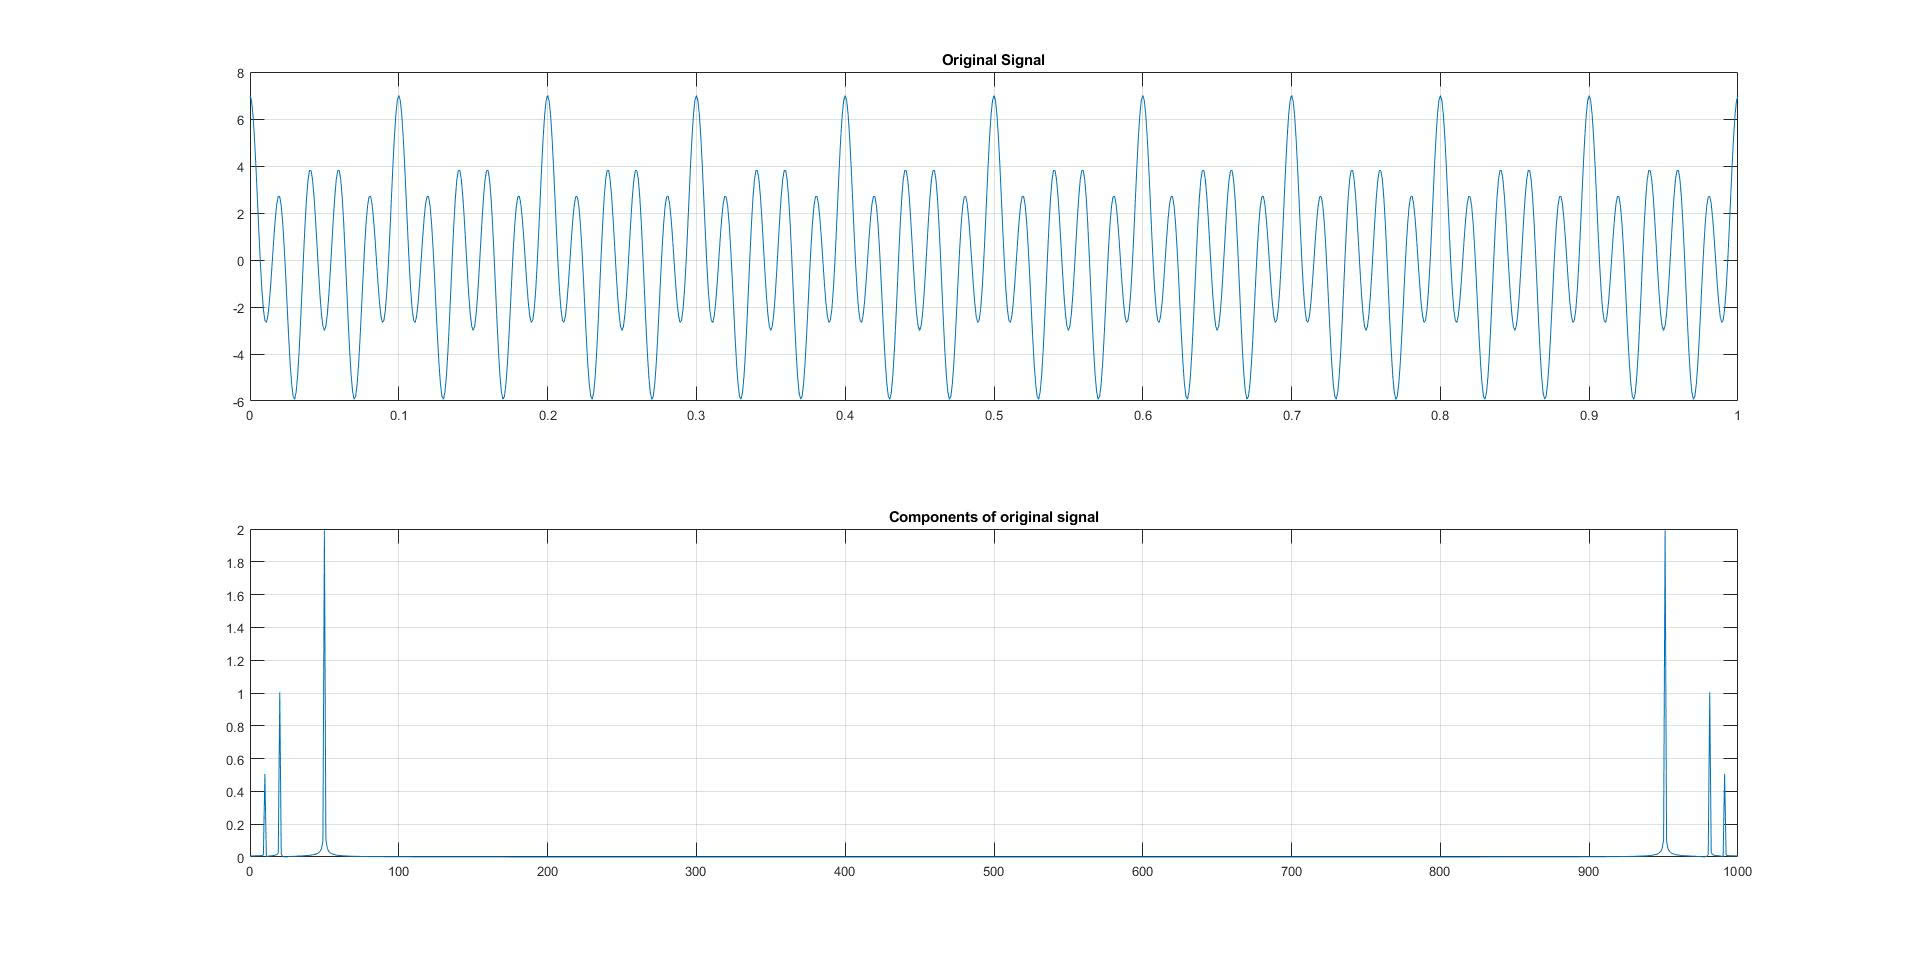
\includegraphics[width=1\textwidth]{original.jpeg}
		\caption{Original signal and its components}
		\label{fig:re3}
	\end{figure}
Ta sử dụng \textbf{phép biến đổi Fourier} (sẽ được học rất kĩ ở chương 3) để tách tín hiệu input vào thành các thành phần điều hòa (harmonic) tuần hoàn với các tần số tương ứng nhất định, được biểu diễn rất rõ trên hình.
\end{frame}
\begin{frame}{Giới thiệu khái quát môn học}
	\begin{figure}[h]
		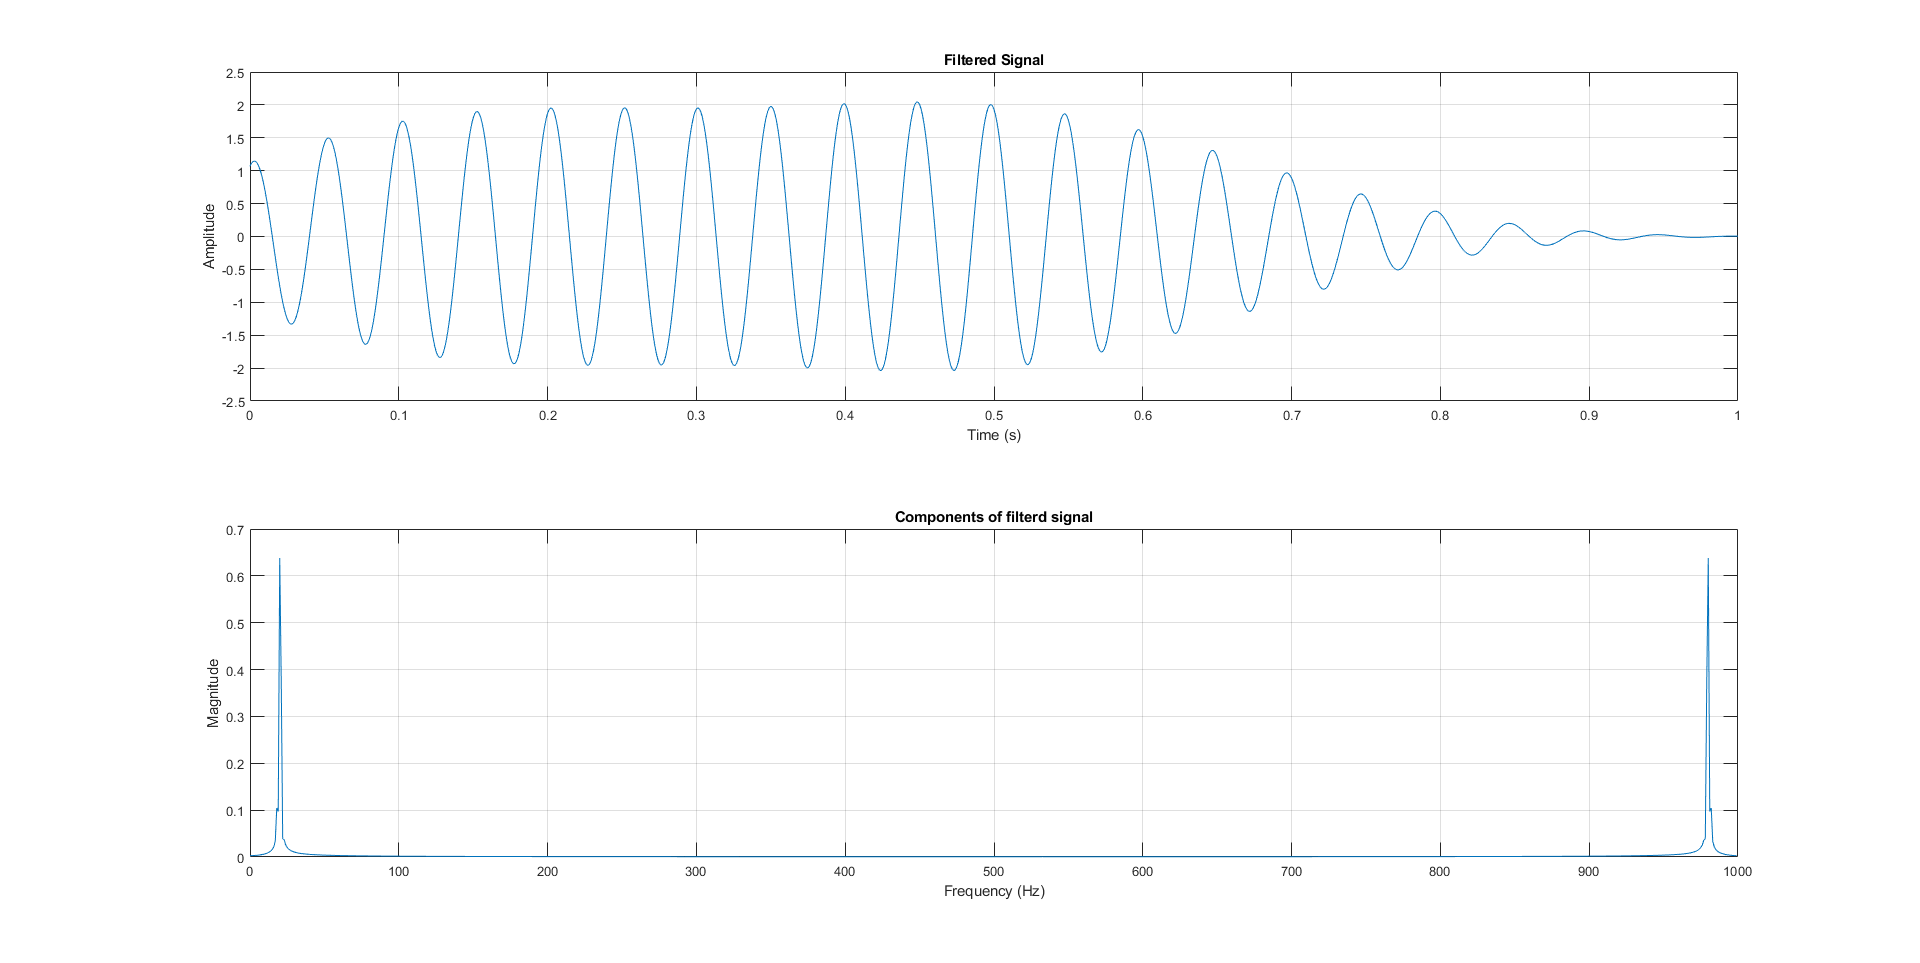
\includegraphics[width=1\textwidth]{filter.png}
		\caption{Filtered signal and its components}
		\label{fig:re4}
	\end{figure}
Giả sử trong trận bóng này, âm thanh gây nhiễu từ cổ động viên và còi tương ứng là 2 "thanh" tần số thứ nhất và thứ ba, và âm thanh của nhà báo thể thao tương ứng có tần số được biểu diễn ở "thanh" thứ hai. Ta cần phải thiết kế hệ thống để loại bỏ hai "thanh" tín hiệu nhiễu sao cho chỉ còn "thanh" của nhà báo.
\end{frame}
\begin{frame}{Kiến thức cơ sở tiên quyết}
	\begin{itemize}
		\item \textbf{Giải tích I} 
			\begin{itemize}
				\item Đây là môn học \textbf{tối quan trọng}, tiên quyết bắt buộc phải \textbf{qua} trước khi học \textbf{Tín hiệu và hệ thống}.
				\item Nếu bạn trượt môn này, hãy học lại cho đến khi \textbf{qua} thì thôi rồi học \textbf{Tín hiệu và hệ thống cũng chưa muộn}. Đừng cố đăng kí học khi bạn trượt \textbf{Giải tích I} nếu bạn không muốn trượt thêm một môn nữa.
			\end{itemize}
		\item \textbf{Giải tích II}
			\begin{itemize}
				\item Kiến thức môn này mặc dù không quá liên quan nhưng tương đối quan trọng khi liên hệ giữa công thức Fubini đổi thứ tự tính tích phân $2$ và $3$ lớp với phép toán đổi thứ tự tính chuỗi vô hạn với tích phân dùng rất nhiều trong môn học này.
				\item Nhìn chung, nếu bạn đã học  môn này thì rất tốt, nhưng nếu chưa học thì cũng không sao cả. 
			\end{itemize}
		\item \textbf{Vật lý đại cương I, II}
			\begin{itemize}
				\item Nội dung môn học này sẽ \textbf{cực kì thú vị} nếu bạn thích Vật lý.
				\item Cũng giống như \textbf{Giải tích II}, nếu bạn học tốt môn này thì rất tuyệt vời, còn không thì cũng không sao cả.
			\end{itemize}
		\item \textbf{Kĩ thuật điện}
			\begin{itemize}
				\item Nếu bạn học chắc môn này, bạn sẽ hiểu được tư tưởng của \textbf{Tín hiệu và hệ thống} mạch lạc và rõ ràng hơn, nhất là sau khi bạn đã hoàn toàn thành thạo với tính toán trên tập $\mathbb{C}$ và giải phương trình vi phân.
				\item Cũng như hai môn học trên, nếu bạn đã học rồi thì rất tốt, còn nếu không thì không sao cả.
			\end{itemize}
	\end{itemize}
\end{frame}
\begin{frame}{Phương pháp học đúng}
	\begin{itemize}
		\item \alert{Phải tự làm hết bài tập về nhà của các thầy/cô, không được đi chép.}
		\item \textbf{Nếu không tự làm bài tập, bạn sẽ không bao giờ có thể "thẩm" nổi môn này !}
		\item Nếu cảm thấy chưa thỏa mãn, hãy làm thêm các bài tập sau (mình cũng đã từng làm qua trong quá trình học) \url{https://shorturl.at/slR55}.
		\item Mình cũng sẽ tìm và lọc các bài tập hay cùng với đề thi cuối/giữa kì của trường mình để chữa cho các bạn nữa. Mình nghĩ các bạn rất nên làm các bài này.
		\item Rất nên đọc textbook và xem Youtube để bổ trợ kiến thức.
	\end{itemize}
\end{frame}
\begin{frame}{Tài liệu tham khảo}
	\begin{itemize}
		\item Tài liệu tham khảo chính: Signals and Systems (2nd edition) Alan V. Oppenheim and Alan S. Willsky.
		\item Tài liệu tham khảo phụ: Bài tập của mình học khóa trước, đề thi các năm cũ,...
		\item Tài liệu tham khảo phụ: Nếu bạn là sinh viên trường mình và muốn học "tủ" nhiều bài thì nên đọc Signals and Systems (2nd edition) Simon Haykin vì các thầy cô chủ yếu dạy và ra đề trong cuốn này, thế nhưng mình đánh giá cuốn này không đầy đủ và chi tiết như sách của Alan V. Oppenheim. 
	\end{itemize}
\end{frame}
\begin{frame}{Ôn tập số phức (optional)}
\end{frame}
\end{document}
